%UNIT 13: SECOND ORDER LINEAR DEs
%%%%%%%%%%%%%%%%%%%%%%%%%%%
%%%% Put the following at the top of each .tex file  %
\pagestyle{fancy}
\renewcommand{\theUnit}{4.2}
\ifthenelse{\isundefined{\UnitPageNumbers}}{}{\setcounter{page}{1}}
\rhead{Section \theUnit: Second Order Linear DEs}
\lhead{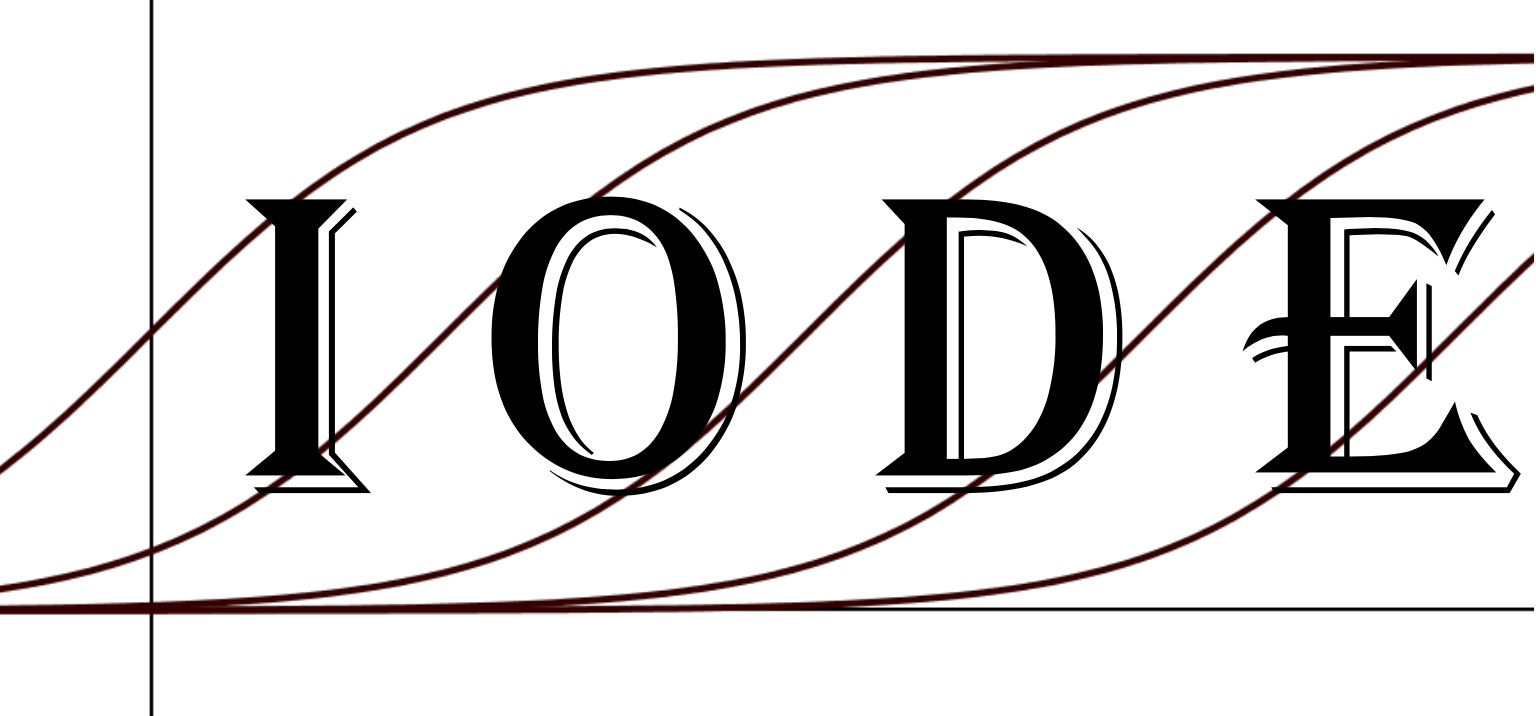
\includegraphics[width=1.25cm]{IODE-logo.png}}
\rfoot{\mypage}
\lfoot{}
\cfoot{}
\fancypagestyle{firstfooter}{\footskip = 50pt}
\renewcommand{\footrulewidth}{.4pt}
%%%%%%%%%%%%%%%%%%%%%%%%%%%
\vspace*{-20pt} \thispagestyle{firstfooter}
\pagebegin{Section 4.2: Second Order Linear Differential Equations}

A second order linear differential equation has the form
\[
P(t)\frac{d^2y}{dt^2}+Q(t)\frac{dy}{dt}+R(t)y=G(t)
\]
where $P$, $Q$, $R$, and $G$ are continuous functions. There are many applications for which this type of differential equation is a useful model. %Your previous work with the spring mass problem was one such example.
Here are some examples. \\

\textbf{Glass Breaking}: You probably have all seen in cartoons or on Mythbusters where a wineglass is broken by singing a particular high-pitched note. The phenomenon that makes this possible is called \textit{resonance}. Resonance results from the fact that the crystalline structures of certain solids have natural frequencies of vibration. An external force of the same frequency will ``resonate'' with the object and create a huge increase in energy. For instance, if the frequency of a musical note matches the natural vibration of a crystal wineglass, the glass will vibrate with increasing amplitude until it shatters. The following is one model for understanding resonance: 
\[
\frac{d^2x}{dt^2}+k^2x=\cos(kt)
\]

\textbf{Tacoma Narrows Bridge}: The Tacoma Narrows Bridge in Washington State was one of the largest suspended bridges built at the time. The bridge connecting the Tacoma Narrows channel collapsed in a dramatic way on Thursday November 7, 1940. Winds of 35-46 miles/hours produced an oscillation which eventually broke the construction. The bridge began first to vibrate torsionally, giving it a twisting motion. Later the vibrations entered a natural resonance (same term as in the glass breaking) with the bridge. Here is a simplified second order differential equation that models the situation of the Tacoma Bridge:
\[
\frac{d^2y}{dt^2}+4y=2\sin(2.1t)
\]

Sometimes resonance is a good thing!  Violins, for instance, are designed so that their body resonates at as many different frequencies as possible, which allows you to hear the vibrations of the strings! \\

There are many other situations that can be modeled with second order differential equations, including mass-spring systems, RLC circuits, pendulums, car springs bouncing, etc. In this section you will learn how to solve second order linear differential equations with constant coefficients. That is, equations where $P$, $Q$, and $R$ are constant. If $G$ is zero, then the equation is called \textbf{homogeneous}. When $G$ is nonzero then the equation is called \textbf{nonhomogeneous}. As you will discover in the sections that follow, the distinction between homogeneous and non-homogeneous equations will be quite useful.

\clearpage

\pagebegin{Guess and Test}

\begin{enumerate}
\item \label{07problem1}
\begin{enumerate}
\item Read the following equations \textit{with meaning}, by completing the following sentence, ``$x(t)$ is a function for which its second derivative ...'' (try saying ``itself'' instead of ``$x$''). \\

\begin{enumerate*}
\item $\displaystyle\frac{d^2x}{dt^2} = -x$ \hspace{.25in}
\item $\displaystyle\frac{d^2x}{dt^2} + x = 0$ \hspace{.25in}
\item $\displaystyle\frac{d^2x}{dt^2} + 4x = 0$ \hspace{.25in}
\item $\displaystyle\frac{d^2x}{dt^2} = x$
\end{enumerate*}

\item For each differential equation above, based on your readings \textit{with meaning}, find two different solution functions. \vfill
\end{enumerate}
\item Your task in this problem is to use the ``guess and test'' approach to find a solution to the linear second order, homogeneous differential equation \label{07problem2}
\[
\frac{d^2x}{dt^2}+10\frac{dx}{dt}+9x=0
\]
By now you know very well that solutions are functions. What is your best guess for a function whose second derivative plus 10 times its first derivative plus 9 times the function itself sum to zero? Explain briefly the rationale for your guess and then test it out to see if it works. If it doesn't work keep trying. \vfill

\item Determine if a constant multiple of your solution is also a solution. \label{07problem3} \vfill

\clearpage

\item Try and find a different solution, one that is not a constant multiple of your solution to problem \ref{07problem2}. \label{07problem4} \vfill

\item Determine the \textit{general solution} to $\displaystyle\frac{d^2x}{dt^2}+10\frac{dx}{dt}+9x=0$. \label{07problem5} \vfill

\clearpage

\item Consider again the differential equation $\displaystyle\frac{d^2x}{dt^2}+10\frac{dx}{dt}+9x=0$. \label{07problem6}

\begin{tabular}{|p{2.5in}|p{3in}|}
\hline
By guessing $x(t) = e^{rt}$, show that this guess yields a solution to the differential equation precisely when $r^2 + 10r + 9 = 0$. \vspace{2.25in} &  \\ \hline
Solve this quadratic equation to find two different values of $r$. \vspace{1.25in} &  \\ \hline
State two different solutions for the differential equation, one for each value of $r$. &  \\ \hline
Form the general solution by multiplying your two solutions by constants $c_1$ and $c_2$, and adding the results. &  \\ \hline
Congratulate yourself :) &  \\ \hline
\end{tabular}

\item Find the general solution to the following differential equation: $\displaystyle\frac{d^2x}{dt^2}+\frac{dx}{dt}-6x=0$. \label{07problem7}


\clearpage

\ii Show $y=Cte^{2t}$ is a solution to $y''-4y'+4y=0$. \vfill

\ii Why do you think the previous example has a ``different'' looking solution? \vspace{2in}


\noindent Solve each of the differential equations below. If initial conditions are given, find the particular solution. 

\ii $z''+z'=z$ \vfill %4.2 Q8 

\clearpage

\ii $3w''+18w'+27w=0$ \vfill %Mine repeated
\ii $w''+8w'+16w=0$; $w(0)=-2$; $w'(0)=12$.  \vfill %Mine repeated
\ii $y'' +3y'-10y=0$; $y(0)=8$, $y'(0)=6$. \vfill %Mine, Real


\end{enumerate}

\end{document}

\clearpage
\pagebegin{The Nonhomogeneous Case}
\begin{enumerate}%[resume]
\item In this next problem your task is to find a solution to the following \textbf{nonhomogeneous} version of the differential equation from the first problem:
\[
\frac{d^2x}{dt^2}+10\frac{dx}{dt}+9x=18.
\]
What is your best guess for a function whose second derivative plus 10 times its first derivative plus 9 times the function itself sum to 18? Test out your guess to see if it works. If it doesn't work keep trying. \label{07problem8}
\end{enumerate}
\clearpage

The solution you found in the previous problem is called the \textbf{particular solution} to the nonhomogeneous differential equation. To find the general solution to the nonhomogeneous differential equation you simply add the particular solution to the general solution to the corresponding homogeneous equation. This 3-step strategy (1 - Find the general solution to the corresponding homogeneous equation; 2 - Find the particular solution to the nonhomogeneous equation, 3 - Add the previous results) is called the \textbf{Method of Undetermined Coefficients}.

\begin{enumerate}[resume]
\item Write down the general solution to $\displaystyle\frac{d^2x}{dt^2}+10\frac{dx}{dt}+9x=18$ and give a convincing argument for why this sum is in fact a solution is the nonhomogeneous differential equation. \label{07problem9} \vfill

\item Sean and Phil are trying to find the particular solution to $\displaystyle\frac{d^2x}{dt^2}+10\frac{dx}{dt}+9x=85\sin(2t)$. Sean guesses $x(t)=A\sin(2t)$ for the particular solution and Phil guesses $x(t)=B\cos(2t)$. \label{07problem10}

\begin{enumerate}
\item Do you think these are reasonable guesses? Explain why or why not. \label{07problem10parta} \vfill
\item For each of their guesses, can you find a value of $A$ or $B$ such that their guess is a solution? If yes, write down the general solution. If no, come up with a different guess for the particular solution and show that your guess is correct. \label{07problem10partb} \vfill
\end{enumerate}

\clearpage

\item Write down the general solution to $\displaystyle\frac{d^2x}{dt^2}+10\frac{dx}{dt}+9x=85\sin(2t)$. \label{07problem11} \vfill

\item Find the general solution to $\displaystyle\frac{d^2x}{dt^2}+10\frac{dx}{dt}+9x=85\sin(2t)$+18. Explain why you can do this by combining results from the previous problems. \label{07problem12} \vfill

\item An aside on complex numbers: \label{07problem07}
\begin{enumerate}
\item Show that $x(s) = e^{is}$ and $x(s) = \cos(s) + i\sin(s)$ are both solutions to the differential equation $dx/ds = ix$ with $x(0) = 1$.  What does the uniqueness theorem imply about these two solutions? \label{07problem07parta} \vfill
\item The above result is called Euler's formula. Multiplying by $e^{\alpha t}$ and using $s =\beta t$, we can rewrite the formula into the following form: $e^{(\alpha + \beta i )t} =  e^{\alpha t} (\cos(\beta t) + i\sin(\beta t))$. Use this to find a similar formula for $e^{(\alpha - \beta i) t}$. \label{07problem07partb} \vfill

\clearpage

\item Suppose you have two functions: \label{07problem07partc}
\begin{align*}
A(t) &= e^{\alpha t} (\cos(\beta t) + i\sin(\beta t)) \\
B(t) &= e^{\alpha t} (\cos(\beta t) - i\sin(\beta t))
\end{align*}
Simplify the following expressions in (i) and (ii) then answer (iii) and (iv).
\begin{enumerate}
\item $x_1(t) = \displaystyle\frac{A(t) + B(t)}{2}$ \label{07problem07partci} \vfill
\item $x_2(t) = i\displaystyle\frac{A(t) - B(t)}{2}$ \label{07problem07partcii} \vfill
\item What do you notice about your solutions in (i) and (ii), compared to $A(t)$ and $B(t)$? \label{07problem07partciii} \vfill
\item If $A(t)$ and $B(t)$ were solutions to a differential equation of the form
\[
a\frac{d^2x}{dt^2} + b\frac{dx}{dt} + cx = 0,
\]
would $x_1(t)$ and $x_2(t)$ be solutions too? How about $c_1x_1(t) + c_2x_2(t)$ for arbitrary constants $c_1$ and $c_2$? \label{07problem07partciv} \vfill
\end{enumerate}
 
\end{enumerate}

\clearpage

\item Find the general solution to the homogeneous differential equation \label{07problem14} 
\[
\frac{d^2x}{dt^2}+25x=0
\]
You will find that your guess results in complex roots to the quadratic.  Use the above results on exponentiation of complex numbers to find the general solution to the differential equation. \vspace{1.75in}

\item \label{07problem15}
\begin{enumerate}
\item Consider the nonhomogeneous differential equation \label{07problem15parta}
\[
\frac{d^2x}{dt^2}+25x=10\cos(5t)
\]
Suppose you wish to find the particular solution to this differential equation. Explain why a guess of the form $x(t) = A\cos(5t) + B\sin(5t)$ is doomed to fail. \vfill
\item Nevertheless, explain why your particular solution must have terms that \textit{look like} $\cos(5t)$ and $\sin(5t)$. \label{07problem15partb} \vfill
\item For an unknown differentiable function $f(t)$, write down the first and second derivatives of $tf(t)$, what do you notice? \label{07problem15partc} \vfill
\item Explain why a guess of $At\cos(5t)$ is insufficient to find the particular solution. \label{07problem15partd} \vfill

\clearpage

\item Use the guess $x(t) = t(A\cos(5t) + B\sin(5t))$ to find a particular solution to the above equation. \label{07problem15parte} \vfill

\end{enumerate}

\item \label{07problem16}
\begin{enumerate}
\item Find the general solution to \label{07problem16parta}
\[
\frac{d^2x}{dt^2}+25x=10\cos(5t).
\]
\vspace{1in}
\item Find the specific solution for initial conditions $x(0)=0$, $x'(0)=1$. \label{07problem16partb} \vfill

\end{enumerate}

\end{enumerate}

\clearpage

\pagebegin{Homework Set 07}

\begin{enumerate}
\item When we are solving a nonhomogeneous second order linear differential equation, the above task sequence had you create a general strategy to first find the solution to the corresponding homogenous equation. You may or may not have found that you always end up solving a quadratic equation to find the coefficients of the exponent variable. In other words, the equation looks like this.
\[
k^2+bk+c=0
\]              
This is called the \textbf{characteristic equation} for the homogeneous linear DE.
Find the characteristic equation and solve to find the general solution for the following homogeneous linear differential equations. \label{07HWproblem1}
\begin{enumerate}
\item $y'' + y' + 12y = 0$
\item $y'' + y' + y = 0$
\item $y'' + 9y = 0$
\end{enumerate} 

\item Find the solution to the following linear second order differential equations. \label{07HWproblem2}
\begin{enumerate}
\item $y'' -4y' = 0$
\item $y'' -4y' = x$
\item $y'' -4y' = x + \sin(x)$
\item $\displaystyle\frac{d^2y}{dx^2}+4\frac{dy}{dx}+4y=2x+3$
\item $y'' - 5y' + 4y = e^{5x}$
\item $y'' - 5y' + 4y = e^{4x}$
\end{enumerate}

\item Find the solution to the initial value problem \label{07HWproblem3}
\[
y''+2y'+2y=0 \quad \text{where} \quad y(\pi/4)=2 \quad \text{and} \quad y'(\pi/4)=-2.
\]

\item Create a table that provides the guess you might make for the particular solution of a second order DE when you are faced with different possible right hand sides of your DE. For example, if the right hand side is general $A\cos(kt)$, what would you guess... etc. \label{07HWproblem4}

\item In everyday life resonance can be a fairly common phenomenon although you may not realize it. Resonance occurs when a system is forced at its natural frequency, leading to a build-up of the amplitude of oscillation and energy. The effect is familiar to most as the high pitched squeal over a PA system caused by microphone feedback. Mathematically, resonance can be seen as a nonhomogeneous second order differential equation whose particular solution is of the same form as the complementary function. To see how this happens, find the general solution to this differential equation: \label{07HWproblem5}
\[
\frac{d^2y}{dt^2}+4y=3\cos(2t)
\]

\clearpage

\item In this question we will interpret the equation $\displaystyle\frac{d^2y}{dt^2} + 4y = 3\cos(2t)$ as an undamped spring-mass system being periodically driven by the force $F(t) = 3\cos(2t)$. \label{07HWproblem6}
\begin{enumerate}
\item Explain why one should expect the spring to eventually break. \label{07HWproblem6parta}
\item Explore the results of adding a small amount of friction to the system. (\textit{Hint}: the new system would be $\displaystyle\frac{d^2y}{dt^2} + b\frac{dy}{dt} + 4y = 3\cos(2t)$, $b>0$) \label{07HWproblem6partb}
\end{enumerate}

\item The Tacoma Narrows Bridge in Washington State was one of the largest suspended bridges built at the time. The bridge connecting the Tacoma Narrows channel collapsed in a dramatic way on Thursday November 7, 1940. Winds of 35-46 miles/hours produced an oscillation which eventually broke the construction. The bridge began first to vibrate torsinonally, giving it a twisting motion. Later the vibrations entered a natural resonance (same term as in the glass breaking) with the bridge. Here is a simplified second order differential equation that models the situation of the Tacoma Bridge: \label{07HWproblem7}
\[
\frac{d^2y}{dt^2}+4y=2\sin(2.1t)
\]
Solve this differential equation and interpret your solution.

\item Suppose you are solving a DE of the following form: \label{07HWproblem8}
\[
y''+by'+cy=A\sin(mt)
\]
Determine the parameters of $m$ that would assure you that you can use a particular solution guess of
\[
y_p=A\sin(mt)+B\cos(mt)
\]
And not
\[
y_p=t(A\sin(mt)+B\cos(mt))
\]
Explain your answer.

\item Use the Internet (or if you are feeling old school, a book) to learn about the technique of \textbf{variation of parameters}, and use it to solve the following two differential equations. In each case, compare your solution with the one you would get through the method of undetermined coefficients. \label{07HWproblem9}
\begin{enumerate}
\item $y'' - y = e^{2t}$
\item $y'' + y = \cos(t)$
\end{enumerate}


\end{enumerate}




